% { % all template changes are local to this group.
%     \setbeamertemplate{navigation symbols}{}
%     \begin{frame}<article:0>[plain,noframenumbering]
%         \begin{tikzpicture}[remember picture,overlay]
%             \node[at=(current page.center)] {
%                 
\includegraphics[keepaspectratio,
%                                  width=0.75\paperwidth,
%                                  height=\paperheight]{LeeLogo}
%             };
%         \end{tikzpicture}
%      \end{frame}
% }

% \setchessboard{
% smallboard,
% showmover=false,
% color=red
% }

% \begin{frame}[fragile]{Ablauf und Ziele von heute}
% \begin{itemize}[<+->]
%     \item Was bisher geschah? (previously im EF-Informatik)
%     \item Herleitung und Diskussion der berühmten Fibonacci-Folge
%     \item Umsetzung rekursiver Programme in Computern
%     \item diverse Anwendungen
% \end{itemize}
% \end{frame}

\begin{frame}[fragile]{Ablauf und Ziele von heute}
\begin{itemize}[<+->]
    \item Was bisher geschah? (previously im EF-Informatik)
    \item Merge Sort Algorithmus 
    \item Laufzeitanalyse von Merge Sort
    \item Merge Sort ist optimal (unter vergleichsbasierten Sortieralgorithmen)
    \item Arbeiten am Game (2. Lektion)
    \item Backtracking und Sudoku (3. Lektion)
\end{itemize}
\end{frame}

\begin{frame}[fragile]{rekursive Berechnung von $5!$}
\begin{align*}
    \textcolor{Red}{5!} &= 5\cdot\underbrace{4\cdot 3\cdot 2\cdot 1}_{\textcolor{Blue}{4!}} \\
    \textcolor{Blue}{4!} &= 4\cdot\underbrace{3\cdot 2\cdot 1}_{\textcolor{Green}{3!}} \\
    \textcolor{Green}{3!} &= 3\cdot\underbrace{2\cdot 1}_{\textcolor{Goldenrod}{2!}} \\
    \textcolor{Goldenrod}{2!} &= 2\cdot\underbrace{1}_{\textcolor{Fuchsia}{1!}} \\
    \textcolor{Orchid}{1!} &= 1\cdot\underbrace{0!}_{1} = 1
\end{align*}
\end{frame}

\begin{frame}[fragile]{rekursive Berechnung von $5!$}
Durch \textit{Rückwertseinsetzen} erhalten wir nun den Wert für $5!$:
\begin{align*}
    \textcolor{Orchid}{1!} &= 1\cdot 0! = 1 \\
    \textcolor{Goldenrod}{2!} &= 2\cdot\textcolor{Orchid}{1!} = 2\cdot 1 = 2 \\
    \textcolor{Green}{3!} &= 3\cdot \textcolor{Goldenrod}{2!} = 3\cdot 2 = 6 \\
    \textcolor{Blue}{4!} &= 4\cdot\textcolor{Green}{3!} = 4\cdot 6 = 24 \\
    \textcolor{Red}{5!} &= 5\cdot\textcolor{Blue}{4!} = 5\cdot 24 = 120.
\end{align*}
\end{frame}

\begin{frame}[fragile]{rekursive Definition von $n!$}
Es sei $n$ eine natürliche Zahl. Dann definieren wir die Fakultät $n!$ von $n$ durch
\[
  n! := 
  \begin{cases}
    1, &\text{falls $n=0$, (Rekursionsanfang)} \\
    n(n-1)!, & \text{falls  $n\geq 1$. (Rekursionsschritt)}
  \end{cases}
\]
\end{frame}

\begin{frame}[fragile]{rekursive Berechnung von $n!$}
\begin{lstlisting}[language=Python]
def factorial(n):
    if n == 0:
        return 1
    else:
        return n * factorial(n - 1)
\end{lstlisting}
\end{frame}

\begin{frame}[fragile]{Definition und Berechnung der Potenz $a^n$}
Sei $a\in\R$ und $n$ eine natürliche Zahl. Wir definieren den Potenzausdruck $a^n$ rekursiv durch
\[
  a^n := 
  \begin{cases}
    1, &\text{falls $n=0$, (Rekursionsanfang)} \\
    a\cdot a^{n-1}, & \text{falls  $n\geq 1$. (Rekursionsschritt)}
  \end{cases}
\]
\end{frame}

\begin{frame}[fragile]{Definition und Berechnung der Potenz $a^n$}
\begin{lstlisting}[language=Python]
def potenz(a, n):
    if n == 0:
        return 1
    else:
        return a * potenz(a, n - 1)
\end{lstlisting}
\end{frame}

\begin{frame}[fragile]{Definition und Berechnung der Potenz $a^n$}
\begin{lstlisting}[language=Python]
def potenz(a, n):
    if n == 0:
        return 1
    else:
        return a * potenz(a, n - 1)
\end{lstlisting}
\end{frame}


\begin{frame}[fragile]{Summe aller Listeneinträge}
In Python ist eine Liste \lstinline|L| von reellen Zahlen gegeben. Schreiben Sie eine Python-Funktion \lstinline|sum_rek(L)|, welche rekursiv die Summe der Zahlen in der Liste berechnet. Es kann angenommen werden, dass die Länge der Liste $\geq 1$ ist.
\begin{lstlisting}[language=Python]
def sum_rek(L):
    if len(L) == 1:
        return L[0]
    else:
        return sum_rek(L[:-1]) + L[-1]
\end{lstlisting}
Dabei ist \lstinline|L[-1]| das hinterste Element der Liste und \lstinline|L[:-1]| die gesamte Liste ohne das hinterste Element.
\end{frame}



\begin{frame}[fragile]{Palindrome}
Ein Wort heisst \textit{Palindrom}, falls das Wort vorwärts und rückwärts genau gleich gelesen wird.\\
Beispiele:
\begin{itemize}
    \item neben
    \item Rentner
    \item Otto
    \item Lagerregal
\end{itemize}
Das \textit{leere Wort}, also das Wort der Länge $0$, ist ebenfalls ein Palindrom. Schreiben Sie ein rekursives Python-Programm, welches entscheidet, ob ein gegebenes Wort \verb|w| ein Palindrom ist oder nicht.
\end{frame}


\begin{frame}[fragile]{Palindrome}
\begin{lstlisting}[language=Python]
def check_palindrom(w):
    w = w.upper()
    if len(wort) <= 1:
        return True
    elif w[0] != w[-1]:
        return False
    return check_palindrom(w[1:-1])
\end{lstlisting}
\end{frame}

\begin{frame}[fragile]{Palindrome}
Lösung von Schafer, Gondorf et al., 2023
\lstset{basicstyle=\ttfamily\scriptsize}
\begin{lstlisting}[language=Python]
def check_palindrom(w):
    return (True if len(w) <= 1 else (check_palindrom(w[1:-1]) if w[0].lower() == w[-1].lower() else False))
\end{lstlisting}
\lstset{basicstyle=\ttfamily\normalsize}
\end{frame}

\begin{frame}[fragile]{Fibonacci-Folge}
In der zweiten Fassung des Buches \textit{Liber abbaci} (Buch der Rechenkunst) beschrieb der italienische Mathematiker \textit{Leonardo da Pisa}, bekannt als \textit{Fibonacci}, das Wachstum einer Kaninchenpopulation. Dies war im Jahre 1202.
\end{frame}


\begin{frame}[fragile]{Fibonacci-Folge}
\begin{itemize}[<+->]
    \item Jedes geschlechtsreife Paar Kaninchen wirft pro Monat genau ein neues Paar Kaninchen (ein Weibchen und ein Männchen). Die Austragungszeit (Dauer der Schwangerschaft) dauert bei Kaninchen also immer genau einen Monat. Jeden Monat kommt also eine neue Generation von Kaninchen zur Welt.
    \item Ein neugeborenes Paar von Kaninchen wird erst am Ende seines ersten Lebensmonats geschlechtsreif und wirft entsprechend erst Ende seines zweiten Lebensmonats sein erstes Paar Kaninchen.
    \item Kein Kaninchen stirbt, verlässt das betrachtete System oder wird, ausser durch Geburt, in das System hineingebracht.
\end{itemize}
\end{frame}


\begin{frame}[fragile]{Fibonacci-Folge}
\begin{itemize}[<+->]
    \item Sei $G_n$ die Anzahl der geschlechtsreifen Kaninchenpaare und $g_n$ die Anzahl der nicht geschlechtsreifen Kaninchenpaare der Generation $n$ für $n\in\N$.
    \item Beachten Sie, dass die gesamte Anzahl der Kaninchenpaare der Generation $n$ damit der Summe $F_n := G_n+g_n$ entspricht.
\end{itemize}
\end{frame}


\begin{frame}[fragile]{Fibonacci-Folge}
Sei $n\in\N$.
\begin{itemize}[<+->]
\item Es gilt
\begin{align*}
    G_{n+2} = G_{n+1} + g_{n+1},
\end{align*}
da die geschlechtsreifen Kaninchen $G_{n+1}$ der Generation $n+1$ auch einen Monat später noch geschlechtsreif sein werden und die nicht geschlechtsreifen Kaninchen $g_{n+1}$ der Generation $n+1$ einen Monat später geschlechtsreif sein werden.
\item Völlig analog begründet man die Gleichung
\begin{align*}
    G_{n+1} = G_{n} + g_{n}.
\end{align*}
\item Offensichtlich gilt zudem
\begin{align*}
    g_{n+2}  = G_{n+1}.
\end{align*}
\end{itemize}
\end{frame}

\begin{frame}[fragile]{Fibonacci-Folge}
Wir haben also drei Gleichungen für die Population:
\begin{align}\label{eq:Fib1}
    \textcolor{Blue}{G_{n+2}} = \textcolor{Red}{G_{n+1}} +  \textcolor{Blue}{g_{n+1}}
\end{align}
\begin{align}\label{eq:Fib2}
    \textcolor{Red}{G_{n+1}} = \textcolor{Red}{G_{n}} + \textcolor{Red}{g_{n}}
\end{align}
\begin{align}\label{eq:Fib3}
    \textcolor{Purple}{g_{n+2}}  = \textcolor{Purple}{G_{n+1}}
\end{align}
Wir setzen nun Gleichung \ref{eq:Fib2} in Gleichung \ref{eq:Fib1} ein und erhalten:
\begin{align*}
    \textcolor{Blue}{G_{n+2}} &= \textcolor{Red}{G_{n}} + \textcolor{Red}{g_{n}} + \textcolor{Blue}{g_{n+1}} \\
    &\iff \\
    \underbrace{\textcolor{Blue}{G_{n+2}} + \textcolor{Purple}{g_{n+2}}}_{F_{n+2}} &= \underbrace{\textcolor{Purple}{G_{n+1}} + \textcolor{Blue}{g_{n+1}}}_{F_{n+1}} + \underbrace{\textcolor{Red}{G_{n}} + \textcolor{Red}{g_{n}}}_{F_n}.
\end{align*}
\end{frame}

\begin{frame}[fragile]{Fibonacci-Folge}
Für die Gesamtzahl der Population der Kaninchenpaare gilt also
\begin{align*}
    F_{n+2} = F_{n+1} + F_{n}
\end{align*}
für alle $n\in\N$. Für Generation $n=0$ definieren wir $G_0:=0$ und $g_0:=0$. Zu Beginn, also in der Generation $n=1$, wird ein erstes Paar von Kaninchen in das System eingeführt. Dieses erste Paar wird erst nach einem Monat geschlechtsreif. Es gilt also $G_1=0$ und $g_1=1$. Somit besteht die Generation $n=2$ immer noch aus nur einem Paar Kaninchen: $G_2=1$ und $g_2=0$. Die Generation $n=3$ aus zwei Paaren: $G_3=1$ und $g_3=1$. Logisch fortgeführt findet man die sogenannte \textit{Fibonacci-Folge}.
\begin{align*}
    &F_0 = 0, F_1 = 1, F_2 = 1, F_3 = 2, F_4 = 3, F_5 = 5, F_6 = 8,\\
    &F_7 = 13, F_8 = 21, F_9 = 34, F_{10} = 55, F_{11} = 89, \ldots
\end{align*}
\end{frame}

\begin{frame}[fragile]{Fibonacci-Folge}
Die Fibonacci-Folge ist somit rekursiv definiert durch
\[
  F_n := 
  \begin{cases}
    0, &\text{falls $n=0$, (Rekursionsanfang)} \\
    1, &\text{falls $n=1$, (Rekursionsanfang)} \\
    F_{n-1} + F_{n-2}, & \text{falls  $n\geq 2$. (Rekursionsschritt)}
  \end{cases}
\]
\end{frame}

\begin{frame}[fragile]{Fibonacci-Folge (iterative Berechnung)}
\begin{lstlisting}[language=Python,caption=iterative Berechnung der Fibonacci-Folge]
def fibonacci_fast(n):
    # Startwerte
    f_0 = 0
    f_1 = 1
    if n == 0:
        return f_0
    elif n == 1:
        return f_1
    
    for k in range(n - 1):
        f_2 = f_1 + f_0
        # Update
        f_0 = f_1
        f_1 = f_2
    return f_2
\end{lstlisting}
\end{frame}

\begin{frame}[fragile]{Fibonacci-Folge (rekursiv, dynamisch)}
Lösung von Pinter, ChatGPT et al., 2026
\begin{lstlisting}[language=Python,caption=rekursive Berechnung der Fibonacci-Folge mit Memoization,numbers=none,basicstyle=\ttfamily\scriptsize]
def fib_recursive(n, memo={}):
    # Basisfälle
    if n <= 1:
        return n
    
    # Prüfen, ob Ergebnis bereits im "Gedächtnis" ist
    if n in memo:
        return memo[n]
    
    # Berechnung und Speicherung im Memo-Dictionary
    memo[n] = fib_recursive(n - 1, memo) + fib_recursive(n - 2, memo)
    
    return memo[n]
\end{lstlisting}
\end{frame}

\begin{frame}[fragile]{Spirale}
\begin{figure}
    \centering
    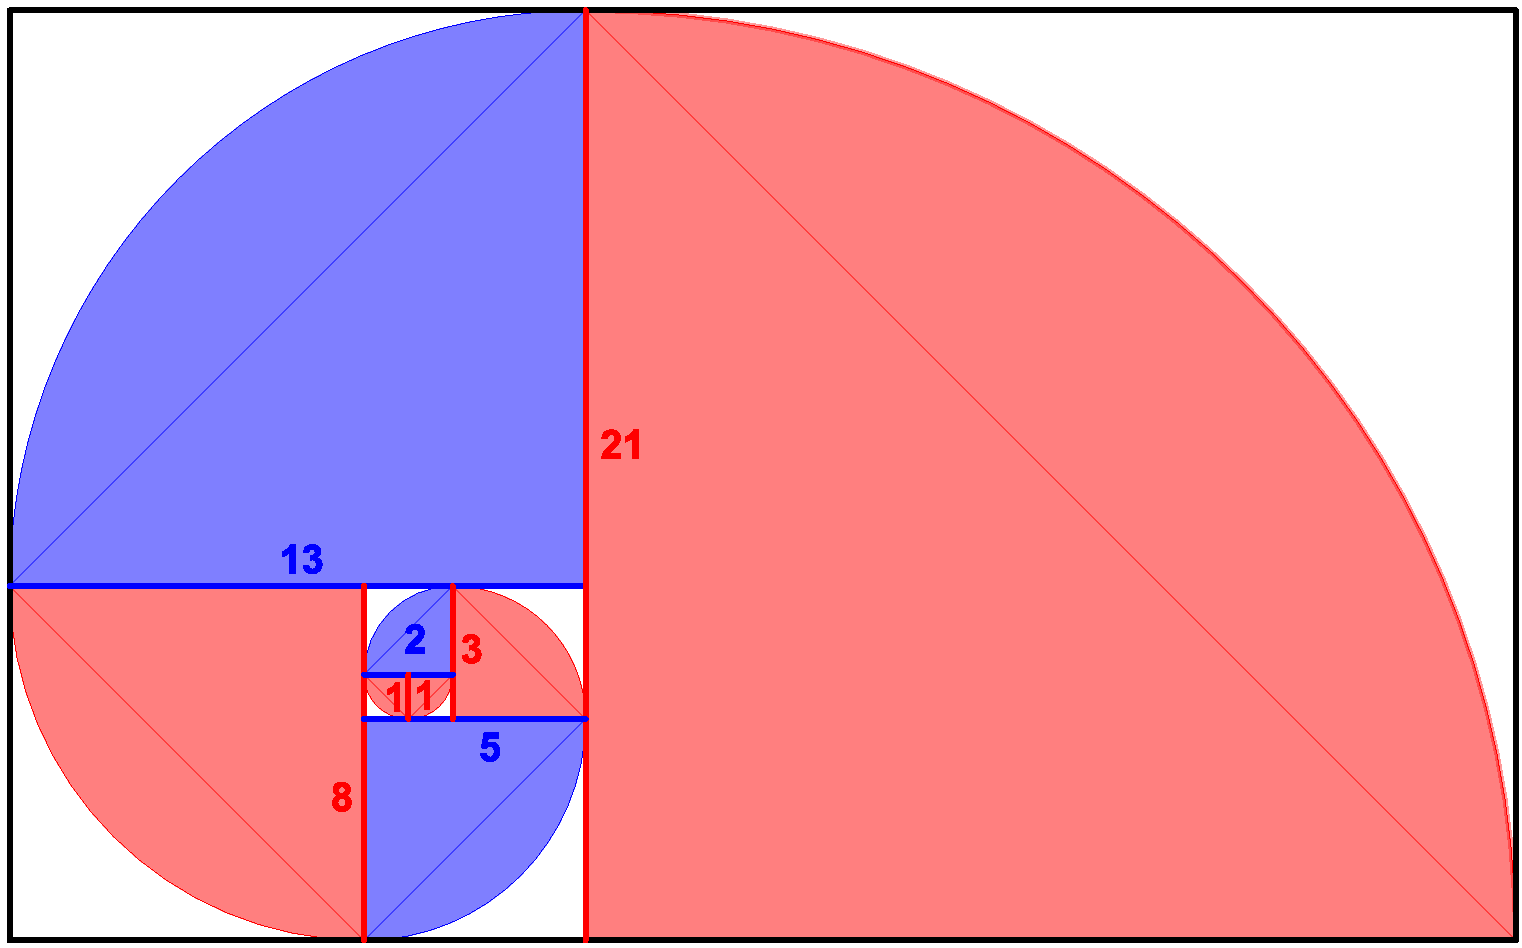
\includegraphics[width=0.6\textwidth]{EF/Induktion_und_Rekursion/Slides/Goldene_Spirale.pdf}
\end{figure}
\end{frame}

\begin{frame}[fragile]
\begin{figure}
    \centering
    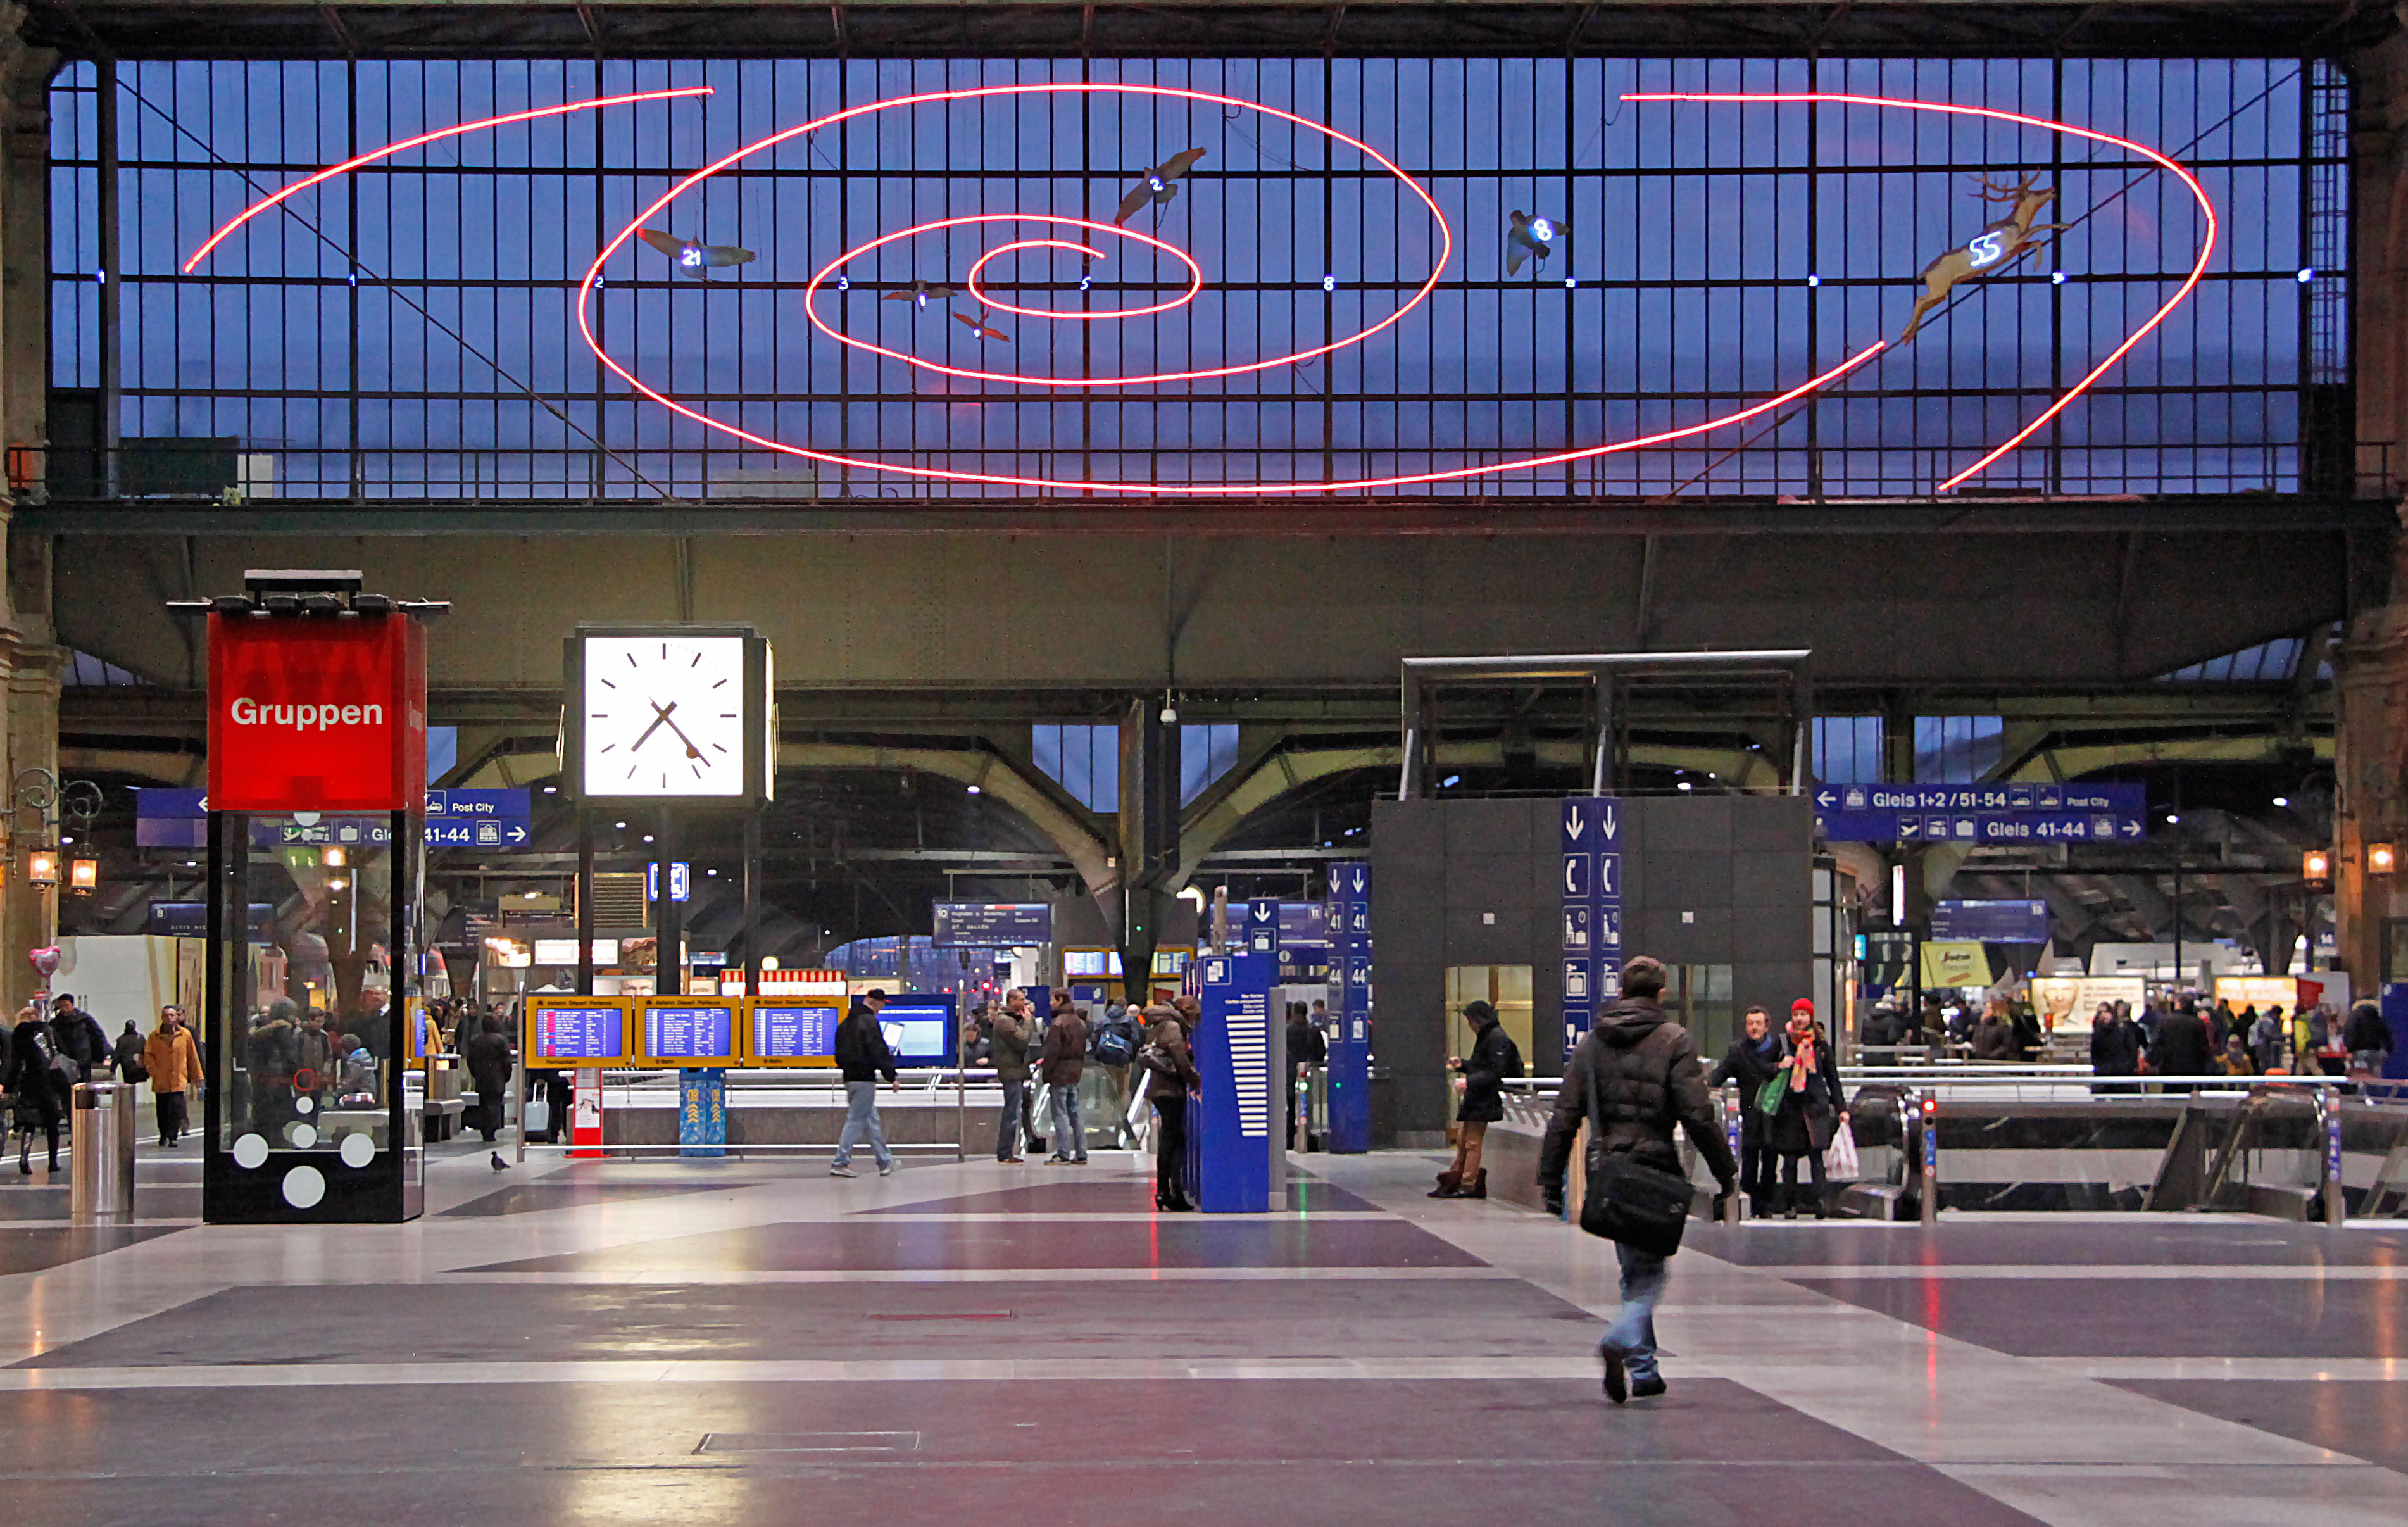
\includegraphics[width=1\textwidth]{EF/Induktion_und_Rekursion/Slides/Fibonacci_numbers_in_Zurich_HB.jpg}
\end{figure}
\end{frame}

% \begin{frame}[fragile]{Aufgaben}
% \begin{itemize}
%     \item Aufgabe 3.11 (A3.7)
%     \item Aufgabe 3.12 (A3.8) $\leftarrow$ die Schnellen können hier die Zeit nutzen, um einen eindrücklichen Plot zu erstellen.
% \end{itemize}
% \end{frame}

% \begin{frame}[fragile]{Fibonacci-Folge auf einem 8-Bit Computer:)}
% \end{frame}

% \begin{frame}[fragile]{Technische Umsetzung rekursiver Programme}
% \begin{lstlisting}[language=Python]
% def binary_strings(n, w = ''):
%     if n == 0:
%         print(w)
%         return
%     binary_strings(n - 1, w + '0')
%     binary_strings(n - 1, w + '1')
%     #return # optional
% \end{lstlisting}
% \end{frame}

% \begin{frame}[fragile]{Binäre Strings ohne aufeinanderfolgende Einsen}
% Bearbeiten Sie Kapitel 4 (Binäre Strings ohne
% aufeinanderfolgende Einsen).
% \end{frame}


\begin{frame}{Problem: Sortieren}
Eines der häufigsten algorithmischen Probleme ist das \textit{Sortieren}.
\begin{mydefinition}[Sortierproblem]\label{mydefinition:Sortierproblem}
Sei $S$ eine Menge, deren Elemente durch die Relation $\leq$ verglichen werden können ($\leq$ heisst dann \textit{totale Ordnung}\footnote{Eine Menge ist total geordnet, wenn für zwei beliebige Elemente $a, b$ aus der Menge immer gilt, dass entweder $a \leq b$ oder $b \leq a$ (oder beides, falls $a=b$).} auf $S$). Das \tib{Sortierproblem}\index{Sortierproblem} lautet dann:
\begin{description}
	\item[Eingabe:] Eine endliche Folge von $n\in\Nunit$ Elementen $a_1, a_2,\ldots, a_n$ aus $S$.
	\item[Ausgabe:] Eine Umordnung $a_1', a_2', \ldots, a_n'$ der Eingabe, sodass $a_1'\leq a_2' \leq \ldots \leq a_n'$ (die Elemente der Eingabe sind nun aufsteigend sortiert).
\end{description}
\end{mydefinition}
\end{frame}


\begin{frame}[fragile]{Sortieren}
\begin{figure}[H]
	\def\lvld{1.2}                  % Choose level distance
	\pgfmathsetmacro\shft{-6*\lvld} % Calculate the yshift for the green tree
	\centering
	\begin{tikzpicture}[
			level distance=\lvld cm,
			level 1/.style={sibling distance=4cm},
			level 2/.style={sibling distance=2cm},
			level 3/.style={sibling distance=1cm},
			edgedown/.style={edge from parent/.style={draw=red,thick,-latex}},
			edgeup/.style={edge from parent/.style={draw=green!50!black,thick,latex-}},
			block/.style={rectangle split, rectangle split parts=#1, draw, fill=blue!20}
		]
		\node[block=7,label={Eingabe},rectangle split horizontal] (A) {3 \nodepart{two} 2 \nodepart{three} 0 \nodepart{four} 3 \nodepart{five} 9 \nodepart{six}8 \nodepart{seven}1};
		
		\node[block=7,right=2cm of A,label={Ausgabe},rectangle split horizontal] (B) {0 \nodepart{two} 1 \nodepart{three} 2 \nodepart{four} 3 \nodepart{five} 3 \nodepart{six}8 \nodepart{seven}9};
		\draw[red,thick,-latex] (A) -- (B);
	\end{tikzpicture}
	\caption{Eingabe und Ausgabe eines kleinen Sortierproblems mit ganzen Zahlen}
	\label{fig:bsp1}
\end{figure}

\begin{figure}[H]
	\def\lvld{1.2}                  % Choose level distance
	\pgfmathsetmacro\shft{-6*\lvld} % Calculate the yshift for the green tree
	\centering
	\begin{tikzpicture}[
			level distance=\lvld cm,
			level 1/.style={sibling distance=4cm},
			level 2/.style={sibling distance=2cm},
			level 3/.style={sibling distance=1cm},
			edgedown/.style={edge from parent/.style={draw=red,thick,-latex}},
			edgeup/.style={edge from parent/.style={draw=green!50!black,thick,latex-}},
			block/.style={rectangle split, rectangle split parts=#1, draw, fill=blue!20}
		]
		\node[block=5,label={Eingabe},rectangle split horizontal] (A) {$r$ \nodepart{two} $e$ \nodepart{three} $a$ \nodepart{four} $o$ \nodepart{five} $n$};
		
		\node[block=5,right=2cm of A,label={Ausgabe},rectangle split horizontal] (B) {$a$ \nodepart{two} $e$ \nodepart{three} $n$ \nodepart{four} $o$ \nodepart{five} $r$};
		\draw[red,thick,-latex] (A) -- (B);
	\end{tikzpicture}
	\caption{Eingabe und Ausgabe eines kleinen Sortierproblems mit Kleinbuchstaben des lateinischen Alphabets. Dabei wurde die übliche alphabetische Ordnung $a\leq b\leq \ldots \leq z$ verwendet.}
	\label{fig:bsp2}
\end{figure}
\end{frame}

\begin{frame}[fragile]{Merge Sort}
\begin{myidea}
Falls zwei jeweils \textbf{bereits sortierte} Listen \lstinline|L| und \lstinline|R| gegeben sind, lassen diese sich recht effizient zu einer (ebenfalls sortierten) Liste \lstinline|M| der Länge $n = \text{len}(L) + \text{len}(R)$ zusammenfügen (englisch: \textit{to merge}).
\end{myidea}

\pause
Beschreiben Sie einen $\Theta(n)$-Algorithmus für den \textit{Merge} zweier sortierter Listen zu einer sortierten Liste.

\end{frame}

\begin{frame}[fragile]{Aufgaben}
\aufgabebox{Lösen Sie \enquote{Aufgaben Rekursion 3} auf Moodle}
\end{frame}


\begin{frame}[fragile]{Merge Sort}
\begin{lstlisting}[language=Python,caption=Implementation von \lstinline|merge_sort|,label=listing:mergesort,numbers=left]
def merge_sort(A):
    # sortiert die Liste A
    if len(A) == 1:  # Rekursionsanfang
        return A  # Listen der Länge 1 sind schon sortiert.

    # teile A in eine linke und rechte Hälfte auf
    if len(A) % 2 == 0:  # falls len(A) gerade ist
        middle = len(A) // 2
    else:  # falls len(A) ungerade ist
        middle = (len(A) // 2) + 1

    L = merge_sort(A[:middle])
    R = merge_sort(A[middle:])
    return merge(L, R)
\end{lstlisting}
\end{frame}

\begin{frame}[fragile]{Ablauf des Algorithmus (\lstinline|merge_sort = ms|, \lstinline|merge = m|)}
\begin{figure}[H]
	\centering
	\begin{tikzpicture}[scale=0.45, every node/.style={scale=0.6},
			->, >=stealth', shorten >=1pt, auto, node distance=3.5cm, semithick]
		\tikzstyle{every state}=[fill=Green!10,draw=black,text=black]

		\node[state] (ms321) {\verb|ms([3,2,1])|};
		\node[state] (ms32) [below left=2.5cm and 1cm of ms321] {\verb|ms([3,2])|};
		\node[state] (ms3) [below left=1.5cm and 1cm of ms32] {\verb|ms([3])|};
		\node[state] (ms2) [below=1.5cm of ms32] {\verb|ms([2])|};
		\node[state,fill=Gold!15] (m32) [below right=1.5cm and 1cm of ms32] {\verb|m([3],[2])|};
		\node[state] (ms1) [below right=2.5cm and 1cm of ms321] {\verb|ms([1])|};
		\node[state,fill=Gold!15] (m231) [right=2.5cm of ms1] {\verb|m([2,3],[1])|};
		\node[above=0.2cm of ms321] {\textcolor{Blue}{$0$ (anfänglicher Aufruf)}};

		\path   (ms321) edge [bend left=15, sloped, midway, above, Blue] node {$1$} (ms32)
		(ms32) edge [bend left=15, sloped, midway, above, Blue] node {$2$} (ms3)
		(ms3) edge [bend left=15, sloped, midway, above, Red] node {$3$} (ms32)
		(ms32) edge [bend left=15, sloped, midway, right, Blue, rotate=-90] node {$4$} (ms2)
		(ms2) edge [bend left=15, sloped, midway, left, Red, rotate=-90] node {$5$} (ms32)
		(ms32) edge [bend left=15, sloped, midway, above, Blue] node {$6$} (m32)
		(m32) edge [bend left=15, sloped, midway, above, Red] node {$7$} (ms32)
		(ms32) edge [bend left, sloped, midway, above, Red] node {$8$} (ms321)

		(ms321) edge [bend left=15, sloped, midway, above, Blue] node {$9$} (ms1)
		(ms1) edge [bend left=15, sloped, midway, above, Red] node {$10$} (ms321)
		(ms321) edge [bend left=10, sloped, midway, above, Blue] node {$11$} (m231)
		(m231) edge [bend left=10, sloped, midway, above, Red] node {$12$} (ms321)
		;
	\end{tikzpicture}
	\caption{schematische Darstellung der Arbeitsschritte von \lstinline{merge_sort}}
	\label{fig:mergesort}
\end{figure}
\end{frame}


\begin{frame}[fragile]{Aufgaben}
\aufgabebox{Lösen Sie \enquote{Aufgaben Rekursion 4} auf Moodle}
\end{frame}


\begin{frame}[fragile]{Laufzeitanalyse von Merge Sort}
    \begin{itemize}[<+->]
        \item Für die nachfolgenden Untersuchungen wollen wir annehmen, dass die Problemgrösse $n$ stets eine Zweierpotenz ist, also $n = 2^k$ für ein $k\in\N$.
        \item Ohne diese Vereinfachungen werden in den Untersuchungen diverse Auf- und Abrundeoperationen notwendig sein und die Darstellung wird technischer und weniger instruktiv.
        \item Zusätzlich möchten wir den trivialen Fall $n = 0$ als Problemgrösse ausschliessen.
    \end{itemize}
\end{frame}

\begin{frame}[fragile]{Laufzeitanalyse von Merge Sort}
Die Laufzeit des \lstinline{merge_sort} Algorithmus setzt sich aus drei einzelnen Teilen zusammen:
\begin{description}[<+->]
	\item[Divide:] Dieser Teil berechnet lediglich die Mitte der zu sortierenden Liste. Dazu ist offensichtlich nur eine konstante Zeit $\Theta(1)$ notwendig.
	\item[Conquer:] Beim Aufruf des \lstinline{merge_sort} Algorithmus mit Problemgrösse $n$ werden rekursiv \textcolor{Blue}{zwei} Teilprobleme (derselben Art) mit jeweils halber Grösse $\textcolor{Green}{n/2}$ aufgerufen. Dies trägt $\textcolor{Blue}{2}T(\textcolor{Green}{n/2})$ zur Laufzeit bei.
	\item[Combine:] Wie wir bereits festgestellt haben, benötigt \lstinline{merge} die lineare Zeit $\Theta(n)$ für die Vereinigung zweier Listen mit summierter Länge \lstinline|n = len(L) + len(R)|.
\end{description}
\end{frame}

\begin{frame}[fragile]{Laufzeitanalyse von Merge Sort}
Zusammengefasst ist die Laufzeit $T(n)$ von \lstinline{merge_sort} im schlimmsten Fall also gegeben durch

\begin{align}\label{eq:rek1}
	T(n) =
	\begin{cases}
		\Theta(1),           & \text{falls $n = 1$,}   \\
		2T(n/2) + \Theta(n), & \text{falls $n\geq 2$}.
	\end{cases}
\end{align}
Gleichung \ref{eq:rek1} lässt sich natürlich schreiben als:
\end{frame}


\begin{frame}[fragile]{Laufzeitanalyse von Merge Sort}
\begin{align}\label{eq:rek2}
	T(n) =
	\begin{cases}
		c_0,            & \text{falls $n = 1$,}   \\
		2T(n/2) + c_1n, & \text{falls $n\geq 2$}.
	\end{cases}
\end{align}
Diesen Ausdruck können wir mit der Definition $c := \max\lrc{c_0,c_1}$ sogar nochmals vereinfachen zu
\begin{align}\label{eq:rek3}
	T(n) =
	\begin{cases}
		c,            & \text{falls $n = 1$,}   \\
		2T(n/2) + cn, & \text{falls $n\geq 2$},
    \end{cases}
\end{align}
da wir uns lediglich für eine obere Schranke interessieren.
\end{frame}


\begin{frame}[fragile]{Laufzeitanalyse von Merge Sort}
\begin{figure}[H]
	\centering
	\begin{tikzpicture}[
			level/.style={sibling distance=40mm/#1},
			text=black,
			>=latex,
			font=\sffamily
		]
		% https://tex.stackexchange.com/questions/241232/creating-dots-lines-brackets-in-tree-with-tikz
		\tikzset{
			edge from parent/.style={draw, thick, black},
			no edge from this parent/.style={
					every child/.append style={
							edge from parent/.style={draw=none}}},
			level 3/.style={yshift=5cm},
			level 4/.style={level distance=5mm}
		}
		\node (z){\textcolor{Red}{$cn$}}
		child {node (a) {\textcolor{Blue}{$cn/2$}}
				child {node  (b) {$cn/4$}
						child {node (b1) {$\vdots$}[no edge from this parent]
								child {node (b11) {$c$}}
							}
						child {node (b2) {$\vdots$}[no edge from this parent]
								child {node (b12) {$c$}}
							}
					}
				child {node (g) {$cn/4$}
						child {node (g1) {$\vdots$}[no edge from this parent]
								child {node (g11) {$c$}}
							}
						child {node (g2) {$\vdots$}[no edge from this parent]
								child {node (g12) {$c$}}
							}
					}
			}
		child {node (d) {\textcolor{Blue}{$cn/2$}}
				child {node  (e) {$cn/4$}
						child {node (e1) {$\vdots$}[no edge from this parent]
								child {node (e11) {$c$}}
							}
						child {node (e2) {$\vdots$}[no edge from this parent]
								child {node (e12) {$c$}}
							}
					}
				child {node (f) {$cn/4$}
						child {node (f1) {$\vdots$}[no edge from this parent]
								child {node (f11) {$c$}}
							}
						child {node (f2) {$\vdots$}[no edge from this parent]
								child {node (f12) {$c$}
									}
							}
					}
			};

		\node[left=5 of z]  (ln1) {$cn$}[no edge from this parent]
		child {node (ln2) {$cn$}[no edge from this parent]
				child {node (ln3) {$cn$}[no edge from this parent]
						child {node (ln4) {}[no edge from this parent]
								child {node (ln5) {$cn$}}}}};

		\coordinate (cd1) at ($(f12)+(1,0)$);
		\coordinate (nb1) at ($(g12)!.5!(e11)$);

		\draw[black,thick,<->,]
		(cd1) --node [fill=white] {$\log(n) + 1$} (cd1|-z.east);

		\draw[black,dashed,thick,->]
		($(z.west)+(-1em,0)$) -- (ln1);
		\draw[black,dashed,thick,->]
		($(a.west)+(-1em,0)$) -- (ln2.east);
		\draw[black,dashed,thick,->]
		($(b.west)+(-1em,0)$) -- (ln3);
		\draw[black,dashed,thick,->]
		($(b11.west)+(-1em,0)$) -- (ln5);

		\draw[Green!70!black,thick,decorate,decoration={brace,amplitude=10pt,mirror}] (b11.south west) --node [below=0.3cm] {$n$} (f12.south east);
	\end{tikzpicture}
	\caption{Laufzeitanalyse von \lstinline{merge_sort}}
	\label{fig:mergesortBaum}
\end{figure}
\end{frame}


\begin{frame}[fragile]{Untere Schranke für das Sortieren durch Vergleiche}
\begin{itemize}[<+->]
    \item Es lässt sich relativ leicht beweisen, dass \lstinline{merge_sort} in einem gewissen Sinne ein optimaler Sortieralgorithmus ist. 
    \item Dies ist einer der Gründe, warum der \lstinline{merge_sort} Algorithmus in Schulen und Universitäten gerne untersucht wird. 
    \item Was meinen wir mit \enquote{in einem gewissen Sinne}? Ein Sortieralgorithmus wird ein (reiner) \textit{vergleichsbasierter} Sortieralgorithmus genannt, falls der Algorithmus lediglich Vergleiche der Form $x \leq y$ verwendet.
    \item Wir wollen beweisen, dass jeder vergleichsbasierte Sortieralgorithmus mindestens $\Theta(n\log(n))$ Vergleiche benötigt, um $n$ Elemente zu sortieren. 
    \item In diesem Abschnitt nehmen wir an, dass alle zu sortierenden Elemente unterschiedlich sind (ohne Beschränkung der Allgemeinheit).
\end{itemize}
\end{frame}


\begin{frame}
\begin{figure}[H]
    \centering
    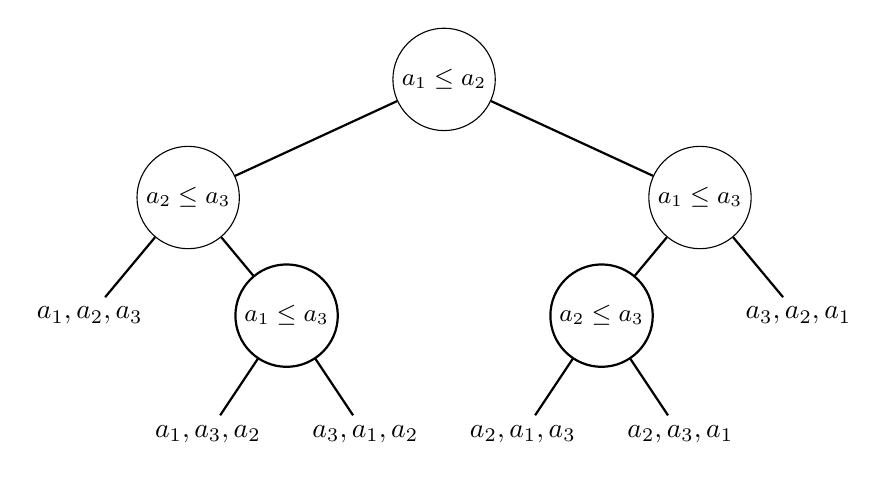
\begin{tikzpicture}[
            level distance=1.5cm,
            % Erhöhte Distanz in Ebene 1, um Platz für die Unterbäume zu schaffen
            level 1/.style={sibling distance=6.5cm},
            % Ebene 2 braucht genug Platz für die Blätter der Ebene 3
            level 2/.style={sibling distance=2.5cm},
            % Ebene 3 verringert, da hier nur Text-Blätter ohne Kreise sind
            level 3/.style={sibling distance=2cm},
            state/.style={circle, draw, minimum size=1.3cm, inner sep=0pt, font=\small}
        ]
        \node[state] {$a_1 \leq a_2$}
            child {node[state] {$a_2 \leq a_3$}
                child {node {$a_1, a_2, a_3$}}
                child {node[state] {$a_1 \leq a_3$}
                    child {node {$a_1, a_3, a_2$}}
                    child {node {$a_3, a_1, a_2$}}
                }
            }
            child {node[state] {$a_1 \leq a_3$}
                child {node[state] {$a_2 \leq a_3$}
                    child {node {$a_2, a_1, a_3$}}
                    child {node {$a_2, a_3, a_1$}}
                }
                child {node {$a_3, a_2, a_1$}}
            };
    \end{tikzpicture}
    \caption{Entscheidungsbaum für das Sortieren von 3 Elementen.}
    \label{fig:decisiontree}
\end{figure}
\end{frame}


\begin{frame}
Ein solcher Baum für $n$ Elemente muss mindestens $n!$ ($n$ Fakultät) Blätter besitzen, da es $n!$ verschiedene Möglichkeiten gibt, $n$ Elemente anzuordnen. Ein binärer Baum der Höhe $h$ hat maximal $2^h$ Blätter. Es muss also gelten:
\begin{align*}
	2^h \geq n! \implies h \geq \log_2(n!)
\end{align*}
Es gilt $\ln(n!) = n \ln n - n + O(\ln(n))$ und somit 
\begin{align*}
	h \geq \log_2(n!) = \Omega(n\log\lr{n}).
\end{align*}
Da \lstinline{merge_sort} eine Laufzeit von $\Theta(n \log\lr{n})$ aufweist, ist dieser Algorithmus asymptotisch optimal.
\end{frame}